\begin{figure*}[t]
\centering
\begin{minipage}{0.245\linewidth}
   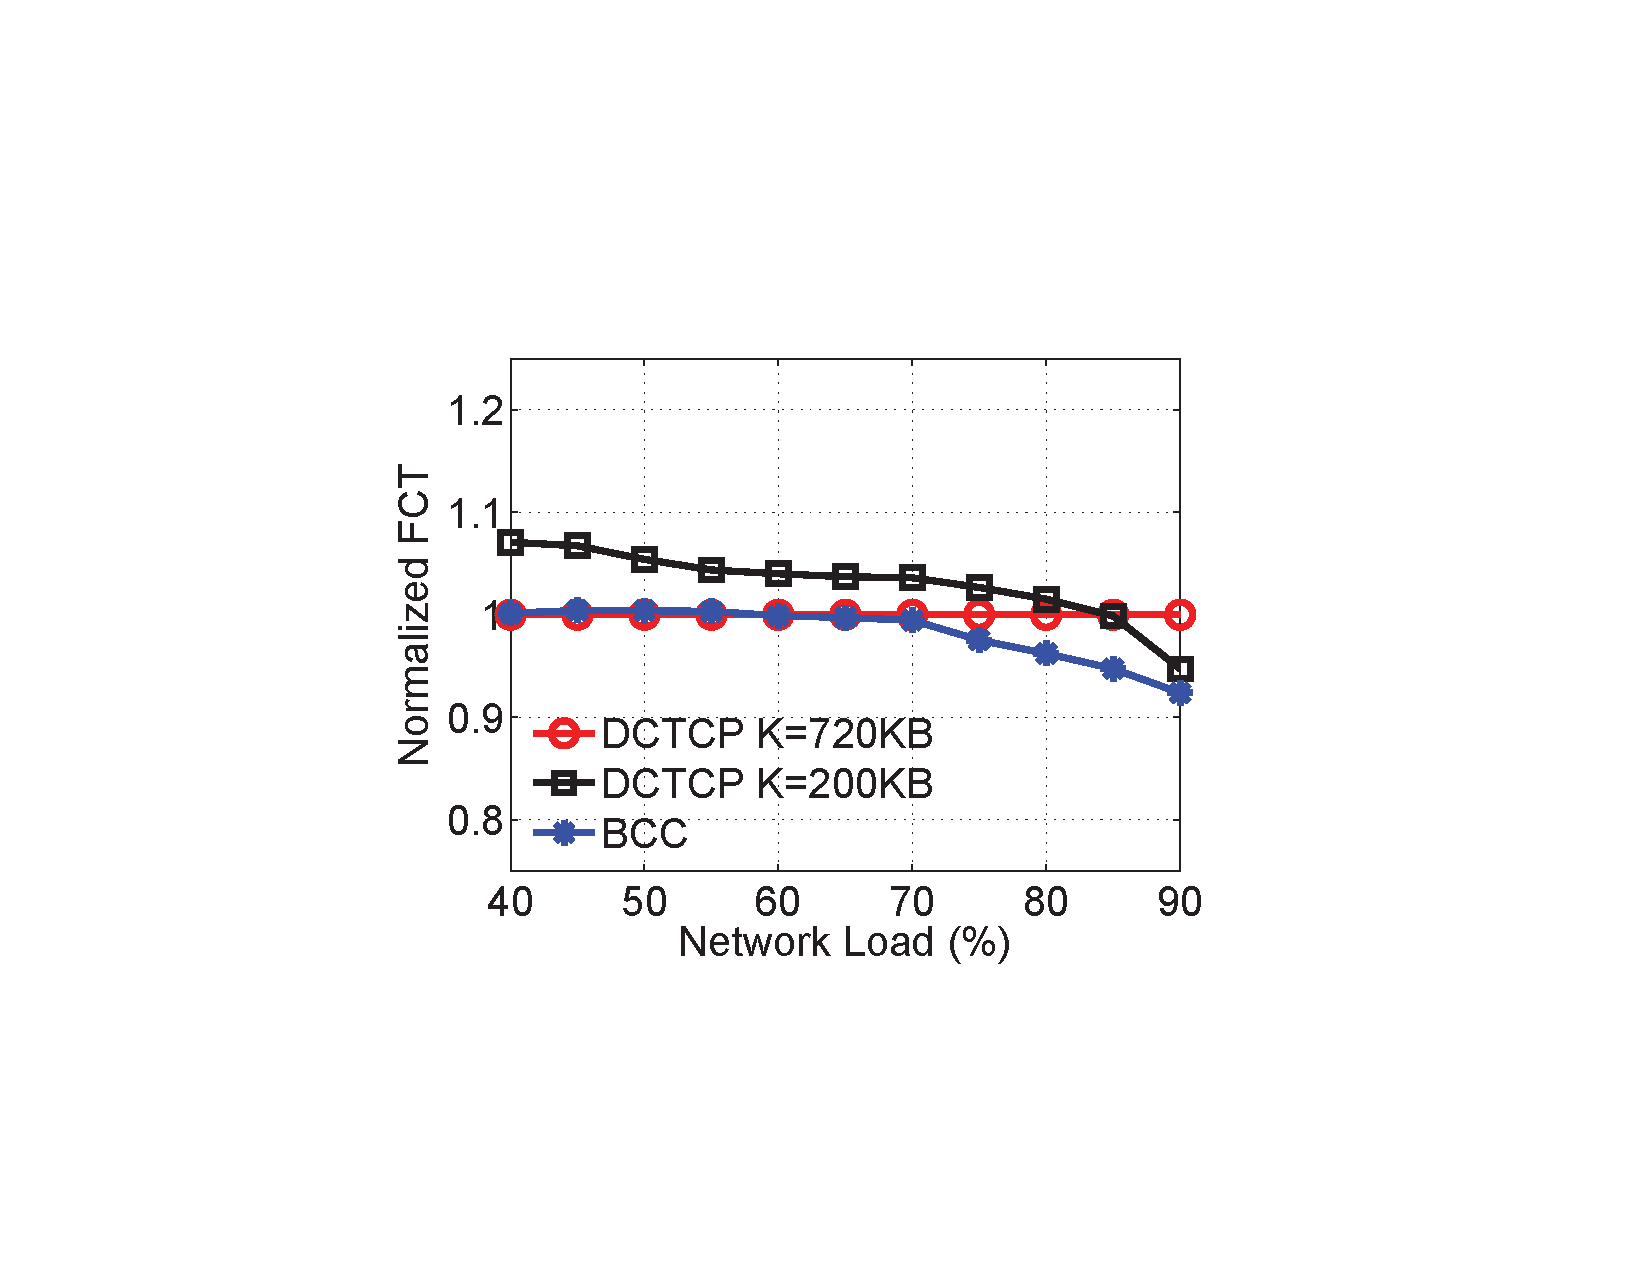
\includegraphics[width=1\linewidth]{figs/websearch_overall_avg_fct.pdf}
   \centerline{(a) Overall: Avg}
\end{minipage}
\begin{minipage}{0.245\linewidth}
   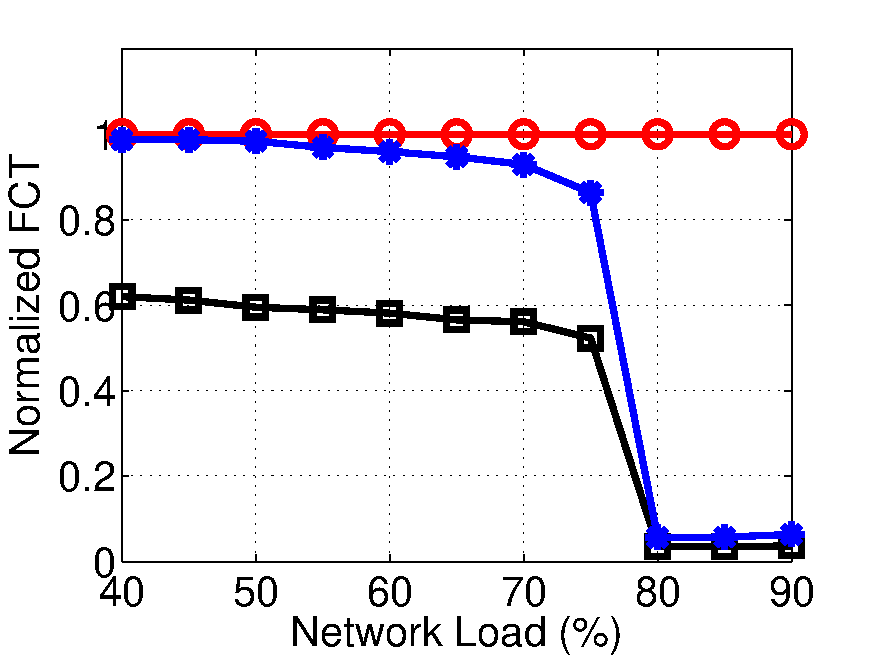
\includegraphics[width=1\linewidth]{figs/websearch_small_tail_fct.pdf}
   \centerline{(b) (0,100KB]: 99th percentile}
\end{minipage}
\begin{minipage}{0.245\linewidth}
   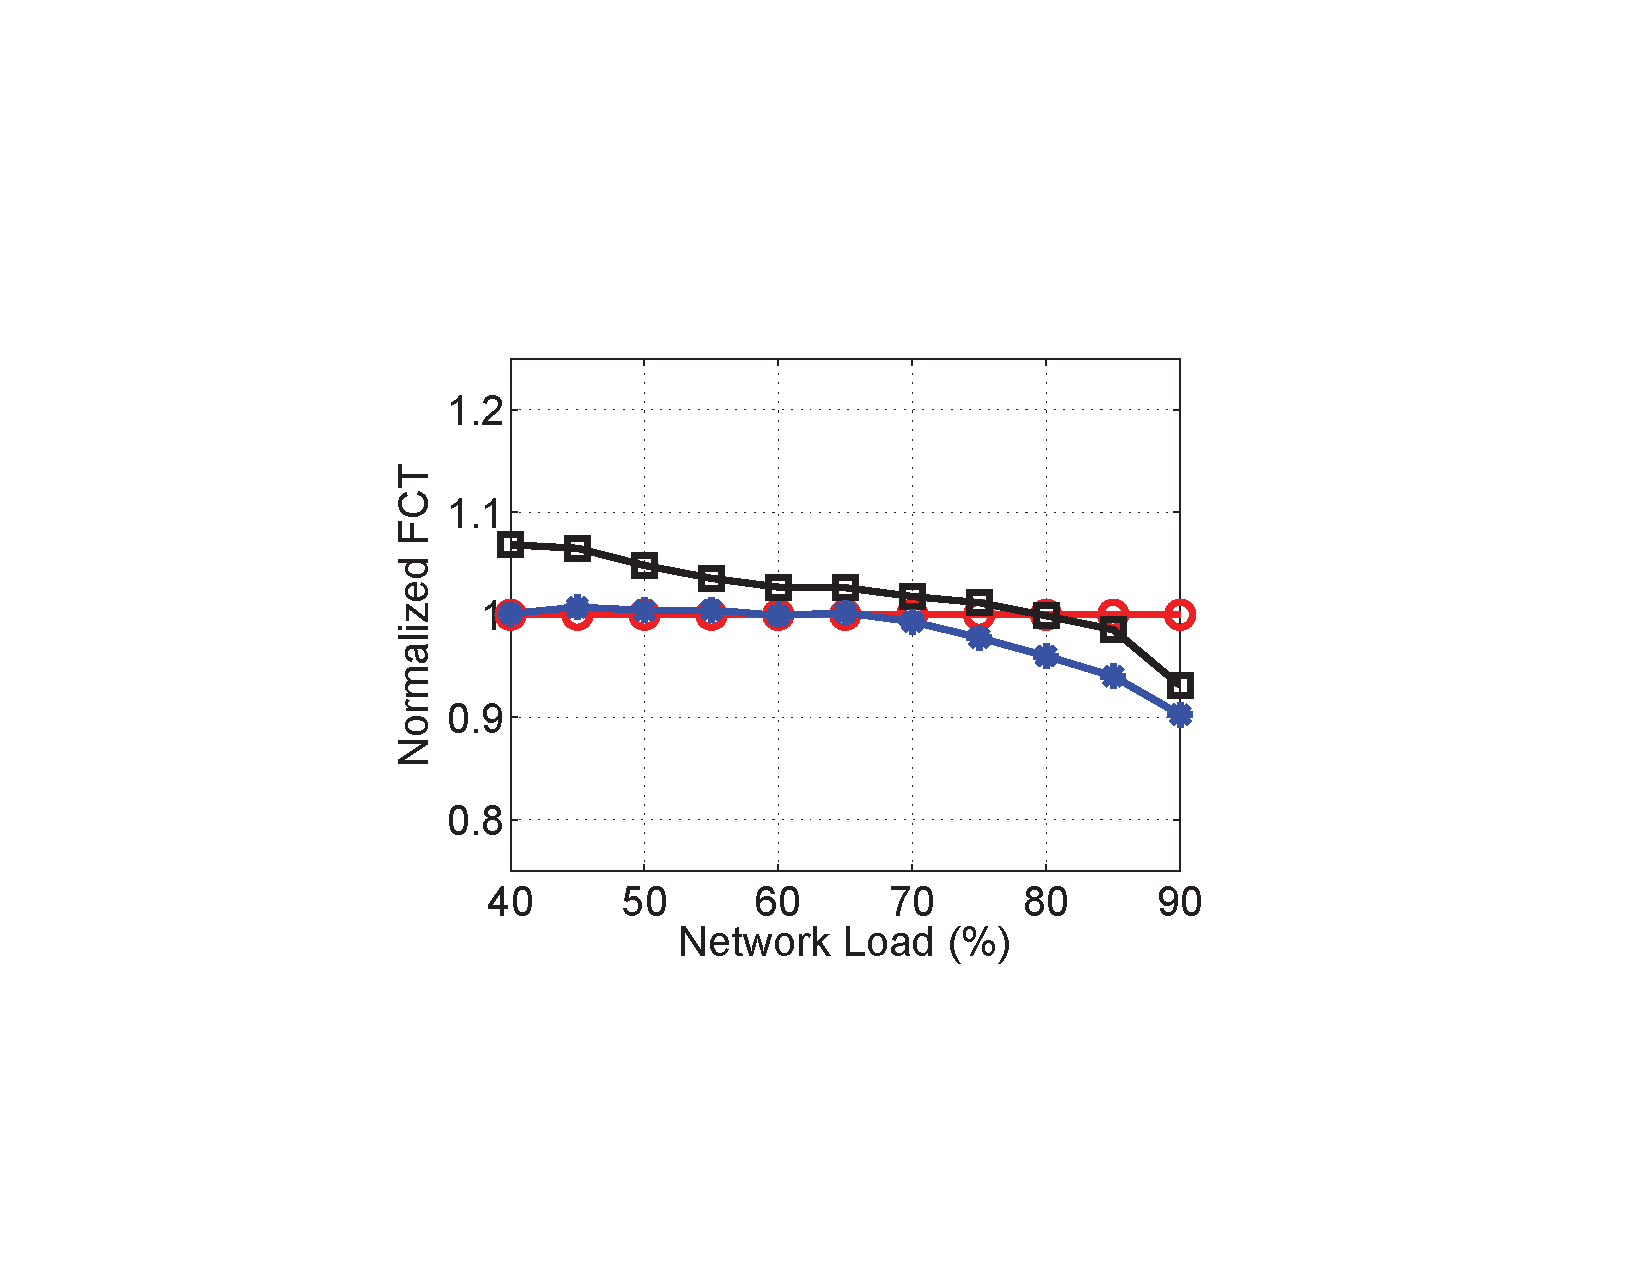
\includegraphics[width=1\linewidth]{figs/websearch_medium_avg_fct.pdf}
   \centerline{(c) (100KB,10MB]: Avg}
\end{minipage}
\begin{minipage}{0.245\linewidth}
   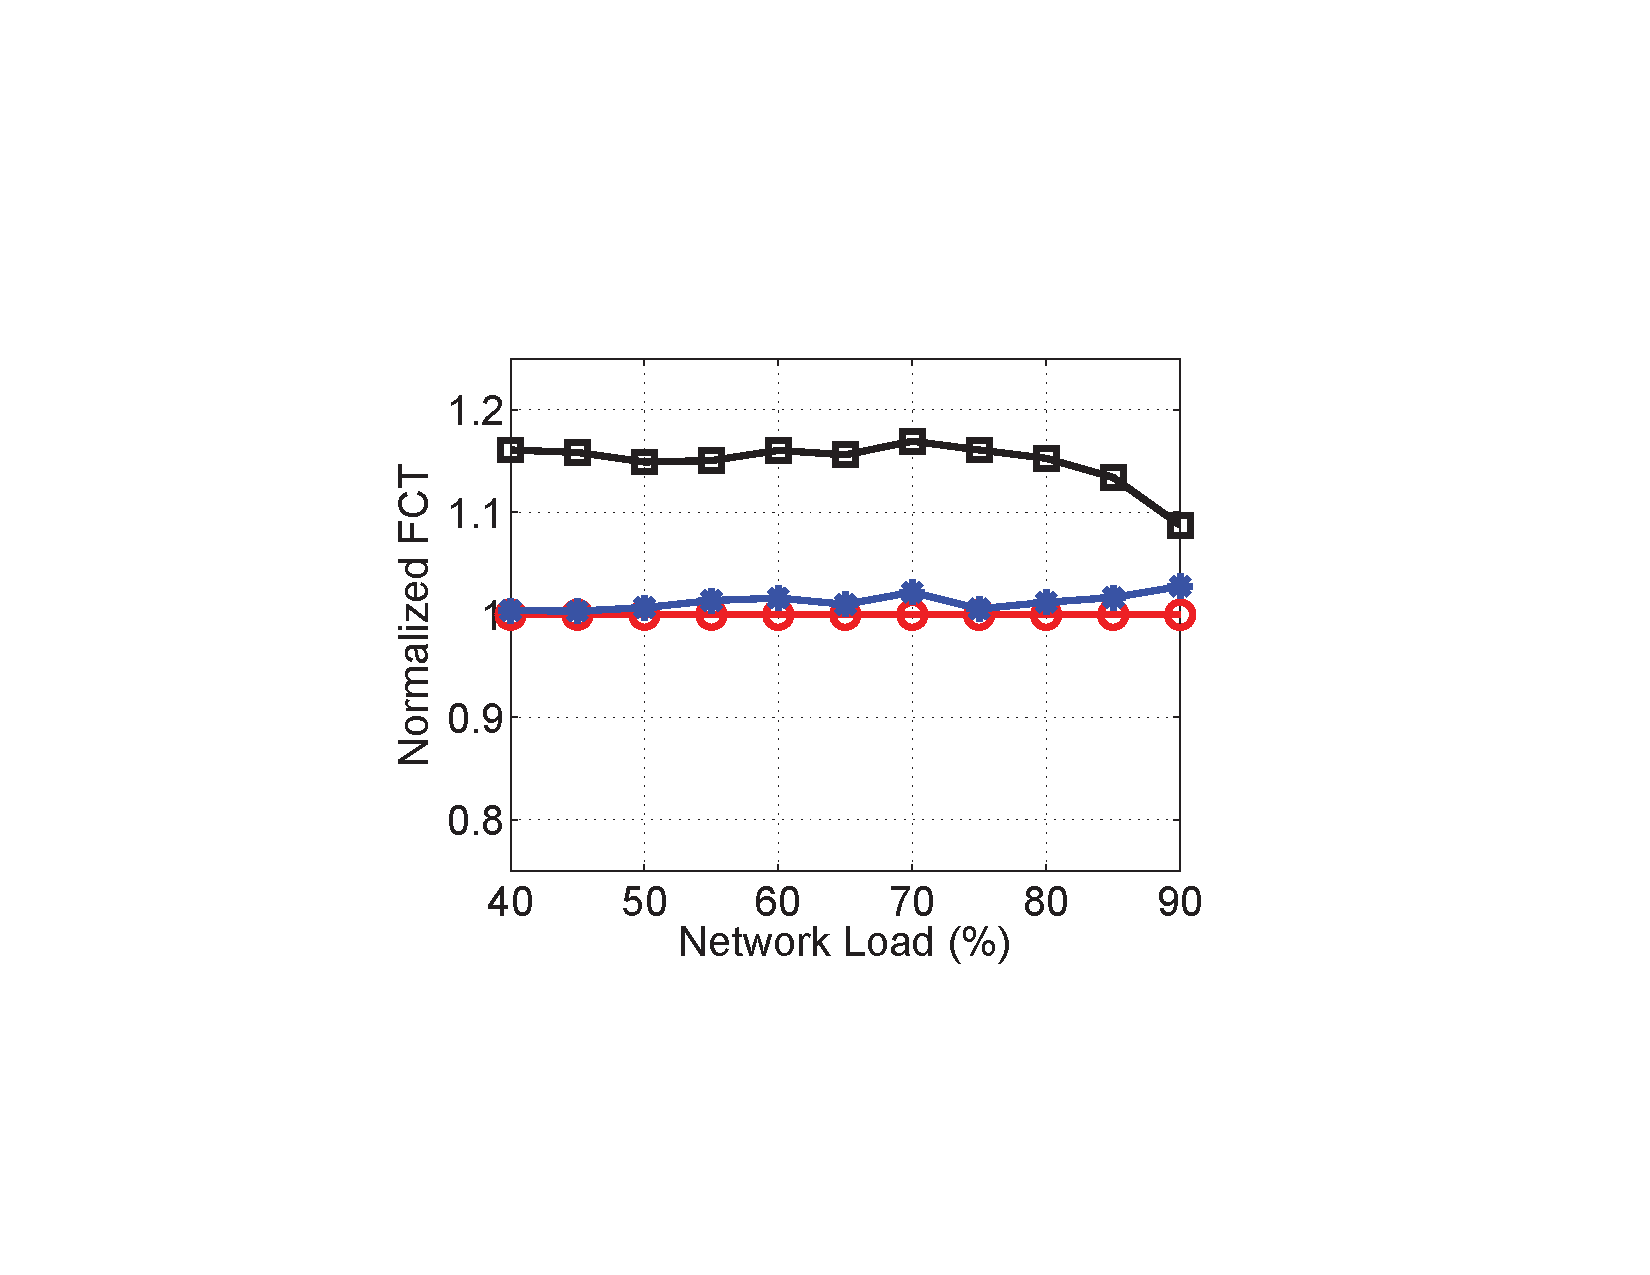
\includegraphics[width=1\linewidth]{figs/websearch_large_avg_fct.pdf}
   \centerline{(d) (10MB,$\infty$): Avg}
\end{minipage}
  \vspace{-2mm}
\caption{[Simulation] Flow Completion Time (FCT) results for the web search workload. Results are normalized to values achieved by DCTCP K=720KB for clear comparison.}\label{fig:websearch_fct}
  \vspace{-3mm}
\end{figure*}
\section{Evaluation}\label{sec:evaluation}
In this section, we present ns-2 simulations results.

\vspace{-1mm}
\parab{Topology:}We simulate a 128-host 100Gbps leaf-spine topology with 8 leaf switches and 8 spine switches. We use ECMP for load balancing. The base fabric RTT is $\sim$80$\mu$s. The BDP is 1MB. The jumbo frame is enabled.

\vspace{-1mm}
\parab{Workload:}We generate traffic according to the web search workload (see~\cite{dctcp} for more details about the distribution). We adjust the flow arrival intervals to achieve the desired load in the network core.

\vspace{-1mm}
\parab{Buffer:}To emulate Tomahawk chip, we attach every 8 switch ports to a 3MB shared buffer pool. We set $\alpha$ to 4 for all ports. In addition, each switch port has 128KB static reserved buffer. We allocate 10MB buffer for each NIC at the host.

\vspace{-1mm}
\parab{Schemes compared:}We use DCTCP~\cite{dctcp} and set RTOmin to 5ms. We compare the following three schemes:
\begin{icompact}
\vspace{-1mm}
\item \textbf{DCTCP K=720KB}: This is a standard ECN configuration (current practice). We configure the per-port (queue) ECN/RED marking threshold to 720KB (0.72BDP based on $\S\ref{subsec:buffer_requirement_high_speed}$) for 100\% throughput.
\vspace{-1mm}
\item \textbf{DCTCP K=200KB}: We configure the per-port (queue) ECN/RED marking threshold to 200KB, which is smaller than average per-port buffer size (512KB), to reduce packet losses.
\vspace{-1mm}
\item \textbf{\sys}: \sys requires two ECN configurations at the switch. We set per-port (queue) ECN/RED marking threshold to 720KB like the standard ECN configuration. Since $\lambda$ is 0.72 for DCTCP and the per-port static reserved buffer size $S_{min}$ is 128KB, $B_R=C\times RTT\times(1+\lambda)-S_{min}\approx$1.6MB. Therefore, $K_{max}\approx$2.6MB, $K_{min}=K_{max}-C\times N\times h\approx$1.8MB and $P_{max}$=10\%.
\end{icompact}

\vspace{-2mm}
\parab{Performance metrics:}We use flow completion time (FCT) as the performance metric and breakdown FCT results across small (0,100KB], medium (100KB,10MB] and large (10MB,$\infty$) flows. Since the performance of many real-time applications depends on the slowest flow, we consider the 99th percentile FCT for small flows.

\vspace{-1mm}
\parab{Result analysis:}According to Figure~\ref{fig:websearch_fct}, we have the following two key observations.
%\vspace{-1mm}
\begin{ecompact}
\vspace{-1mm}
\item At low loads, \sys performs similar as K=720KB while generally outperforming K=200KB, especially for medium and large flows. With the sufficient buffer resource, \sys can fully utilize the link capacity without triggering shared buffer ECN/RED. By contrast, K=200KB still conservatively marks packets, thus significantly degrading throughput. Compared to K=200KB. \sys achieves up to $\sim$13.5\% (6362$\mu$s to 5503$\mu$s) lower average FCT for large flows. K=200KB only shows some performance advantage ($\sim$100$\mu$s) on small flows, due to its lower switch queueing.
\vspace{-1mm}
\item At high loads, \sys generally outperforms the other two schemes. For small flows, \sys achieves up to  94.4\% (5174$\mu$s to 291$\mu$s) lower 99th FCT compared to K=720KB. This is because K=720KB causes excessive packet losses due to the exorbitant shared buffer utilization. The packet loss rate with K=720KB exceeds 0.3\% at 90\% load. This results in frequent TCP timeouts, which seriously increases FCT by at least 5ms (RTOmin). By contrast, at 90\% load, the packet loss rate with \sys is lower than 0.08\%.

    For large flows, \sys's performance is within $\sim$0.4-2.8\% of the K=720KB. This suggests that \sys only slightly degrades large flows. We think that the lower packet loss rate with \sys can make up for throughput loss to some degree. By contrast, DCTCP K=200KB is still so conservative that it increases FCT by at least $\sim$9\% compared to K=720KB.
\end{ecompact}
%In summary, \sys can operate based on the real-time shared buffer utilization, thus keeping good performance in various scenarios.


